\subsection{Dual Quaternion Skinning}
Da Linear Blend Skinning, wie diskutiert, ubiquit�r eingesetzt wird aber oft zu Artefakten f�hrt, kann man laut \cite{kavan2008geometric} diesen Algorithmus leicht durch Erweiterung des linearen Ansatz Dual Quaternionen optimieren und mit minimalen Aufwand aufwerten. 

\begin{figure}[t]
	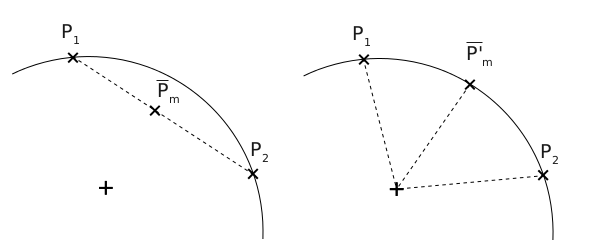
\includegraphics[width=7cm]{01_Skinning/pics/interpolation_angle.png}
	\caption[Vergleich im zweidimensionalen Raum]{ Darstellung im zweidimensionalen euklidischen Raum. Entnommen von \cite{kavan2008geometric}.}
	\label{weights_fig1}
\end{figure}

In Abbildung 9 ist eine vereinfachte Darstellung im zweidimensionalen euklidischen Raum zu sehen. In Linear Blend Skinning vergleicht man essentiell die durchschnittliche Position, an der ein Punkt liegen m�sste. Das f�hrt, wie hier zu sehen ist, unter Umst�nden zu Volumenverlust und damit zu Artefakten. Vergleicht man hingegen, wie rechts, die durchschnittlichen Winkel, kann man Volumenverlust vermeiden.

Ein Weg, dies zu erreichen, ist von \cite{kavan2008geometric}, genannt Dual Quaternion Linear Blending. Ein Quaternion ist im Prinzip ein Vektor mit einer Drehachse. Weiteres nachzulesen hier \cite{dam1998quaternions}. Jede Dual-Zahl wird wie folgt dargestellt: $a + \varepsilon b$ wobei $\varepsilon^2 = 0$ ist. Ein Dual Quaternion kann also einfach als $\mathbf{\dot q} = \mathbf q_0 + \varepsilon \mathbf q_e$ bezeichnet werden. Wie in \cite{kavan2008geometric} bewiesen, kann jede 4*4 Matrize, und damit jede Translation und Transformation, als Dual Quaternion dargestellt werden, womit sich folgende Formel nach \cite{kavan2008geometric} ergibt: 

\begin{equation}
\label{formel}
\mathbf{\dot q} =  \frac{\sum_{i=1}^n w_i \mathbf{\dot q}_i}{\| \sum_{i=1}^n w_i \mathbf{\dot q}_i \|}
\end{equation}

Wir machen also statt einer Verschmelzung aus Transformations-Matrizen, eine aus Dual Quaternionen, wie gewohnt gewichtet. Anschlie�end wird mit ${\| \sum_{i=1}^n w_i \mathbf{\dot q}_i \|}$ normalisiert. Am Schluss der Gleichung erhalten wir ein neues Dual Quaternion, mit dem wir den Punkt auf dem Gittergraphen verschieben k�nnen. Auf Abbildung 10, erkennt man das bei Linear Blend Skinning vorgestellte Problem, auf Abbildung 11 mit Dual Quaternion Blend Skinning.
\begin{figure}[t]
	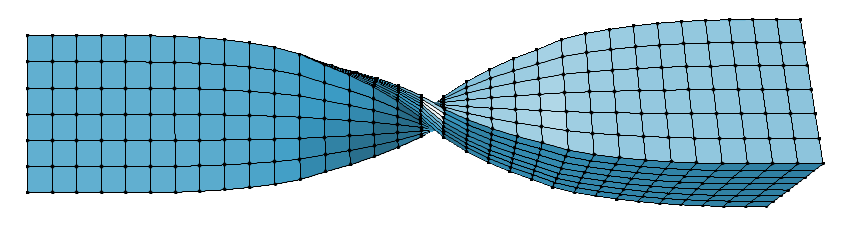
\includegraphics[width=9cm]{01_Skinning/pics/lbsgrad.png}
	\caption[180� Rotation LBS]{ 180� Rotation LBS. Entnommen von \cite{weights}}
	\label{weights_fig1}
\end{figure}

\begin{figure}[t]
	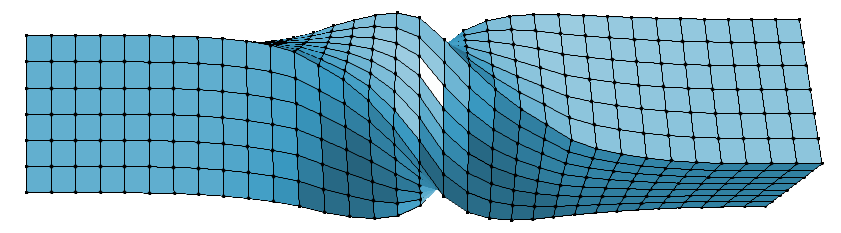
\includegraphics[width=9cm]{01_Skinning/pics/dqsgrad.png}
	\caption[180� Rotation DQS]{180� Rotation DQS. Entnommen von\cite{weights}}
	\label{weights_fig1}
\end{figure}

Der gro�e Vorteil dieser Herangehensweise ist die Vermeidung von Artefakten bei �hnlicher Geschwindigkeit wie beim Linear Blend Skinning. Auch die Implementierung ist nur unwesentlich schwieriger.

Nachteilhaft ist allerdings, dass dieser Algorithmus in manchen F�llen mehr Speicher verbrauchen kann \cite{kavan2008geometric}. Dazu kommt, dass dieser Algorithmus nur feste Transformationen beherrscht, also zum Beispiel keine Skalierung. \cite{kavan2008geometric} Dies wirkt im ersten Moment nicht schlimm, weil reale Personen kein Volumen verlieren. Im Film ist es allerdings durchaus denkbar, dass ein Charakter sein Volumen oder die Gr��e einzelner K�rperteile ver�ndern kann, wodurch bei diesem Ansatz im schlimmsten Fall ein v�llig neues Modell erstellt werden m�sste. Einfacher w�re es vermutlich, f�r diese Bewegungen einen anderen Algorithmus zu verwenden. Ein weiteres Problem ist, dass bei Drehungen an einem Gelenk um mehr als 180� das k�rzeste Weg zu Artefakten f�hren kann. \cite{kavan2008geometric} Dargestellt in Abbildung 12. 

\begin{figure}[tb]
	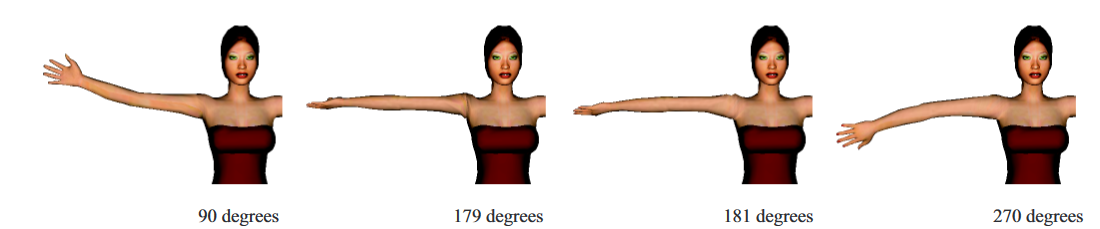
\includegraphics[width=13cm]{01_Skinning/pics/dqsgradartefakte.png}
	\caption[Artefakte DQS bei mehr als 180� Rotation]{Artefakte DQS bei mehr als 180� Rotation Entnommen von \cite{kavan2008geometric}}
	\label{weights_fig1}
\end{figure}
